\section{Dika Sukma Pradana(1174050)}
\subsection{LeafletJs bersama Map Proxy}
\begin{enumerate}
 \item Sesuaikan direktorinya dengan milik kita
    \hfill\break
    \begin{figure}[H]
		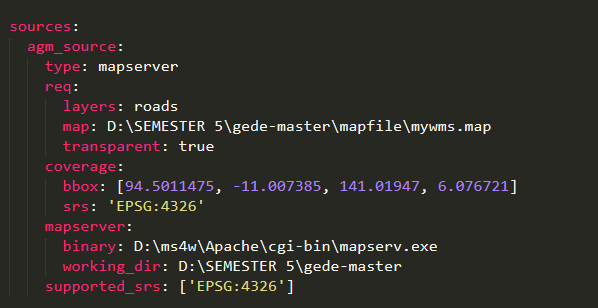
\includegraphics[width=12cm]{figures/1174050/tugas5/2.PNG}
		\centering
		\caption{Penyesuaian Direktori}
	\end{figure}
    \item Run Map Proxy dengan perintah mapproxy-util serve-develop agm.yaml
    \hfill\break
    \begin{figure}[H]
		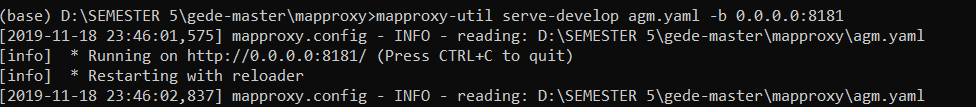
\includegraphics[width=12cm]{figures/1174050/tugas5/1.PNG}
		\centering
		\caption{Run MapProxy}
	\end{figure}
    \item Buka file basic.html di chrome sesuai direktorinya
    \hfill\break
    \begin{figure}[H]
		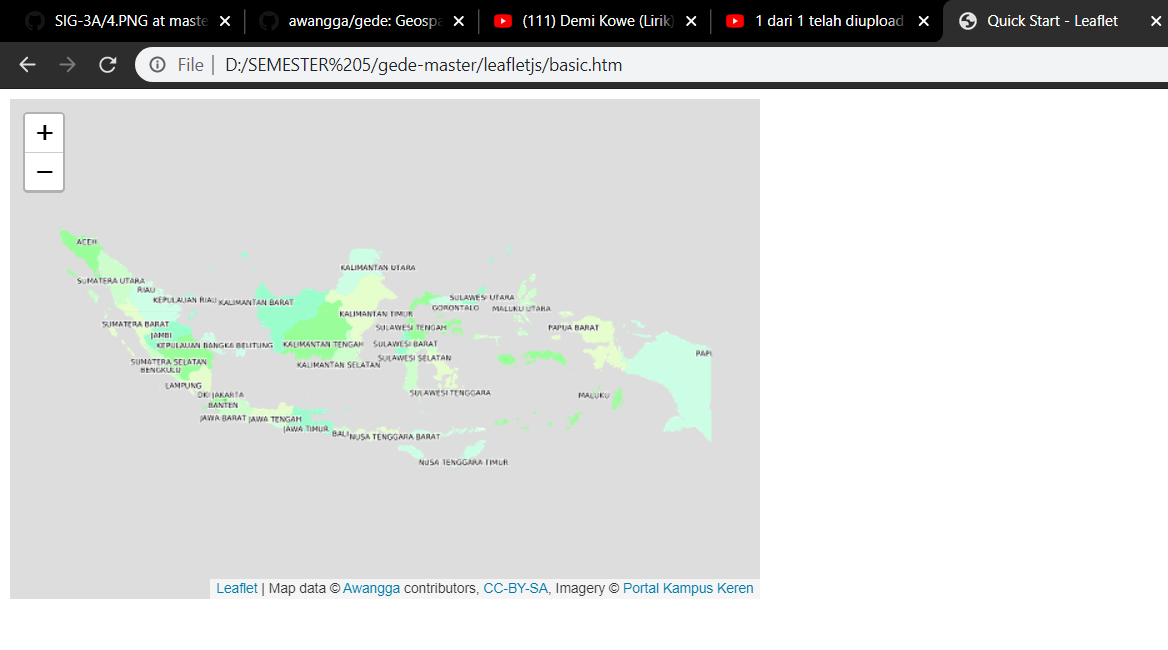
\includegraphics[width=12cm]{figures/1174050/tugas5/3.PNG}
		\centering
		\caption{Buka di Chrome}
	\end{figure}
    \item Pada file marker.html sudah ditambahkan marker pada daerah tertentu
    \hfill\break
    \begin{figure}[H]
		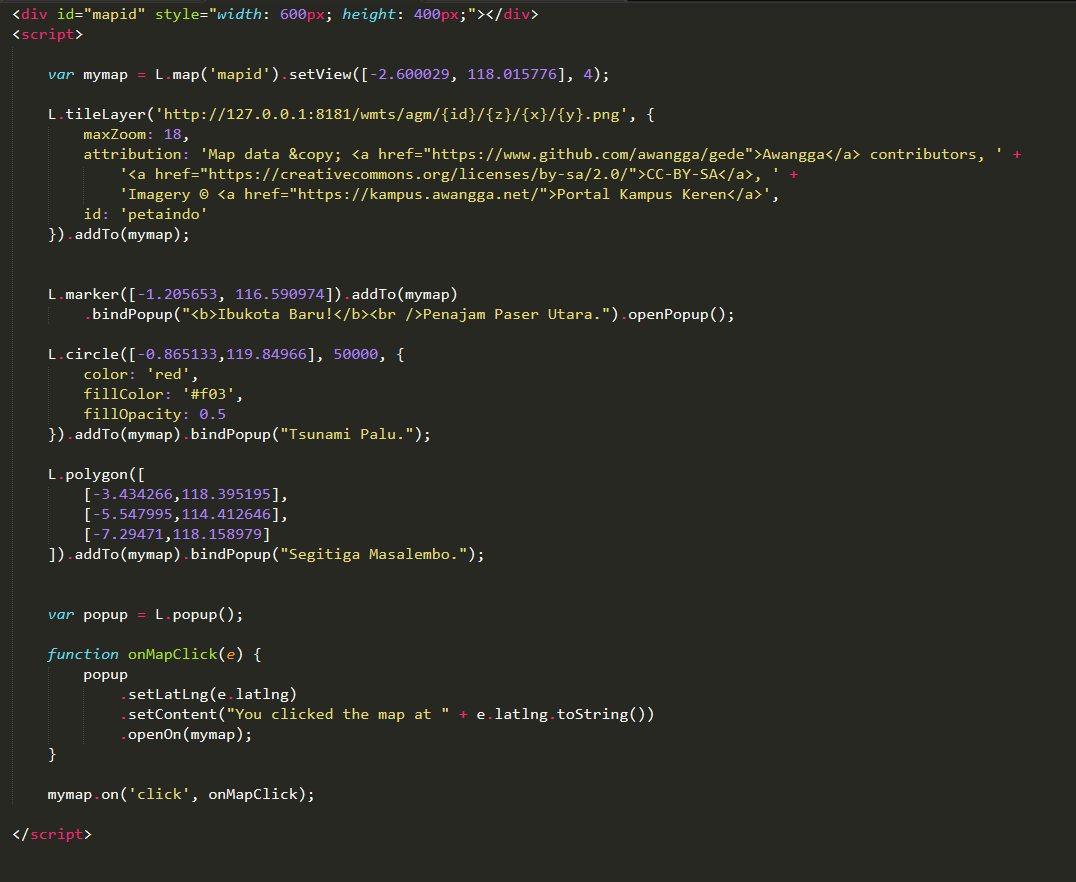
\includegraphics[width=12cm]{figures/1174050/tugas5/4.PNG}
		\centering
		\caption{Tambah Marker}
	\end{figure}
    \item Buka marker.html di browser
    \hfill\break
    \begin{figure}[H]
		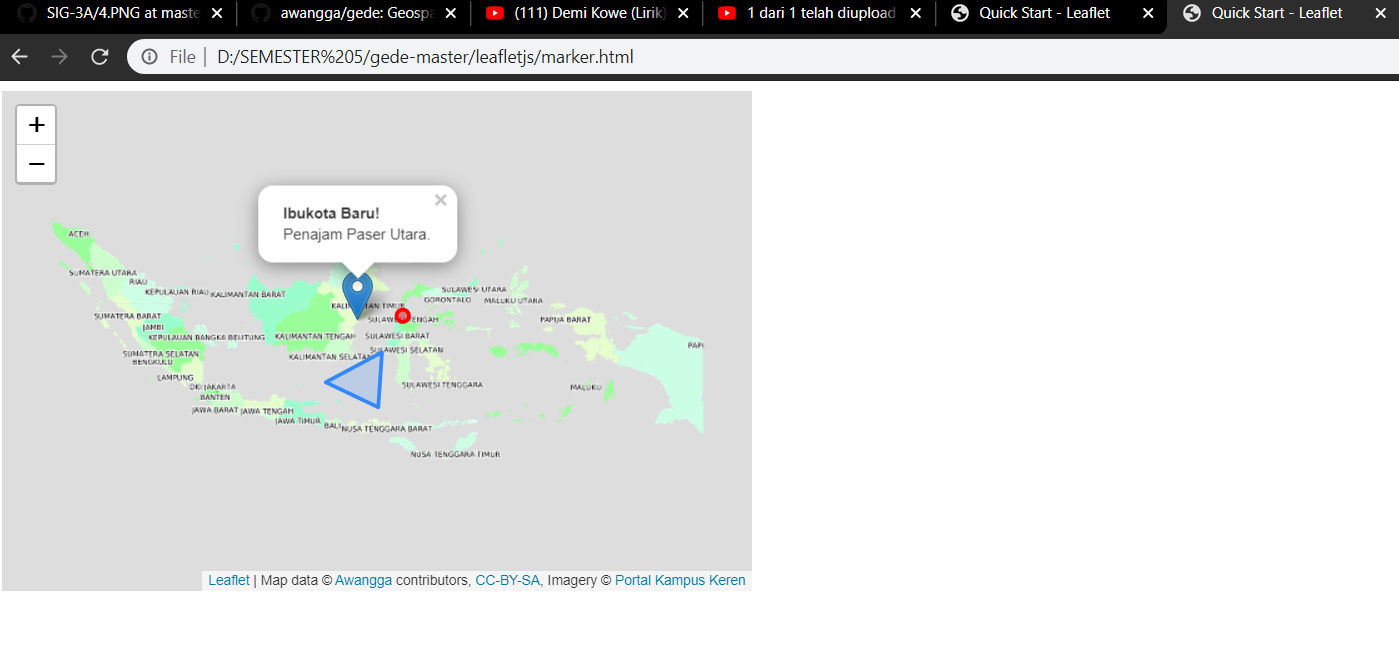
\includegraphics[width=12cm]{figures/1174050/tugas5/5.PNG}
		\centering
		\caption{Tampilan di Browser}
	\end{figure}
\end{enumerate}
\subsection{Link Youtube}
\href{https://youtu.be/1eIGj9vYuS4}{YOUTUBE!JANGAN LUPA SESKREB!}